\documentclass[1p]{elsarticle_modified}
%\bibliographystyle{elsarticle-num}

%\usepackage[colorlinks]{hyperref}
%\usepackage{abbrmath_seonhwa} %\Abb, \Ascr, \Acal ,\Abf, \Afrak
\usepackage{amsfonts}
\usepackage{amssymb}
\usepackage{amsmath}
\usepackage{amsthm}
\usepackage{scalefnt}
\usepackage{amsbsy}
\usepackage{kotex}
\usepackage{caption}
\usepackage{subfig}
\usepackage{color}
\usepackage{graphicx}
\usepackage{xcolor} %% white, black, red, green, blue, cyan, magenta, yellow
\usepackage{float}
\usepackage{setspace}
\usepackage{hyperref}

\usepackage{tikz}
\usetikzlibrary{arrows}

\usepackage{multirow}
\usepackage{array} % fixed length table
\usepackage{hhline}

%%%%%%%%%%%%%%%%%%%%%
\makeatletter
\renewcommand*\env@matrix[1][\arraystretch]{%
	\edef\arraystretch{#1}%
	\hskip -\arraycolsep
	\let\@ifnextchar\new@ifnextchar
	\array{*\c@MaxMatrixCols c}}
\makeatother %https://tex.stackexchange.com/questions/14071/how-can-i-increase-the-line-spacing-in-a-matrix
%%%%%%%%%%%%%%%

\usepackage[normalem]{ulem}

\newcommand{\msout}[1]{\ifmmode\text{\sout{\ensuremath{#1}}}\else\sout{#1}\fi}
%SOURCE: \msout is \stkout macro in https://tex.stackexchange.com/questions/20609/strikeout-in-math-mode

\newcommand{\cancel}[1]{
	\ifmmode
	{\color{red}\msout{#1}}
	\else
	{\color{red}\sout{#1}}
	\fi
}

\newcommand{\add}[1]{
	{\color{blue}\uwave{#1}}
}

\newcommand{\replace}[2]{
	\ifmmode
	{\color{red}\msout{#1}}{\color{blue}\uwave{#2}}
	\else
	{\color{red}\sout{#1}}{\color{blue}\uwave{#2}}
	\fi
}

\newcommand{\Sol}{\mathcal{S}} %segment
\newcommand{\D}{D} %diagram
\newcommand{\A}{\mathcal{A}} %arc


%%%%%%%%%%%%%%%%%%%%%%%%%%%%%5 test

\def\sl{\operatorname{\textup{SL}}(2,\Cbb)}
\def\psl{\operatorname{\textup{PSL}}(2,\Cbb)}
\def\quan{\mkern 1mu \triangleright \mkern 1mu}

\theoremstyle{definition}
\newtheorem{thm}{Theorem}[section]
\newtheorem{prop}[thm]{Proposition}
\newtheorem{lem}[thm]{Lemma}
\newtheorem{ques}[thm]{Question}
\newtheorem{cor}[thm]{Corollary}
\newtheorem{defn}[thm]{Definition}
\newtheorem{exam}[thm]{Example}
\newtheorem{rmk}[thm]{Remark}
\newtheorem{alg}[thm]{Algorithm}

\newcommand{\I}{\sqrt{-1}}
\begin{document}

%\begin{frontmatter}
%
%\title{Boundary parabolic representations of knots up to 8 crossings}
%
%%% Group authors per affiliation:
%\author{Yunhi Cho} 
%\address{Department of Mathematics, University of Seoul, Seoul, Korea}
%\ead{yhcho@uos.ac.kr}
%
%
%\author{Seonhwa Kim} %\fnref{s_kim}}
%\address{Center for Geometry and Physics, Institute for Basic Science, Pohang, 37673, Korea}
%\ead{ryeona17@ibs.re.kr}
%
%\author{Hyuk Kim}
%\address{Department of Mathematical Sciences, Seoul National University, Seoul 08826, Korea}
%\ead{hyukkim@snu.ac.kr}
%
%\author{Seokbeom Yoon}
%\address{Department of Mathematical Sciences, Seoul National University, Seoul, 08826,  Korea}
%\ead{sbyoon15@snu.ac.kr}
%
%\begin{abstract}
%We find all boundary parabolic representation of knots up to 8 crossings.
%
%\end{abstract}
%\begin{keyword}
%    \MSC[2010] 57M25 
%\end{keyword}
%
%\end{frontmatter}

%\linenumbers
%\tableofcontents
%
\newcommand\colored[1]{\textcolor{white}{\rule[-0.35ex]{0.8em}{1.4ex}}\kern-0.8em\color{red} #1}%
%\newcommand\colored[1]{\textcolor{white}{ #1}\kern-2.17ex	\textcolor{white}{ #1}\kern-1.81ex	\textcolor{white}{ #1}\kern-2.15ex\color{red}#1	}

{\Large $\underline{12a_{0823}~(K12a_{0823})}$}

\setlength{\tabcolsep}{10pt}
\renewcommand{\arraystretch}{1.6}
\vspace{1cm}\begin{tabular}{m{100pt}>{\centering\arraybackslash}m{274pt}}
\multirow{5}{120pt}{
	\centering
	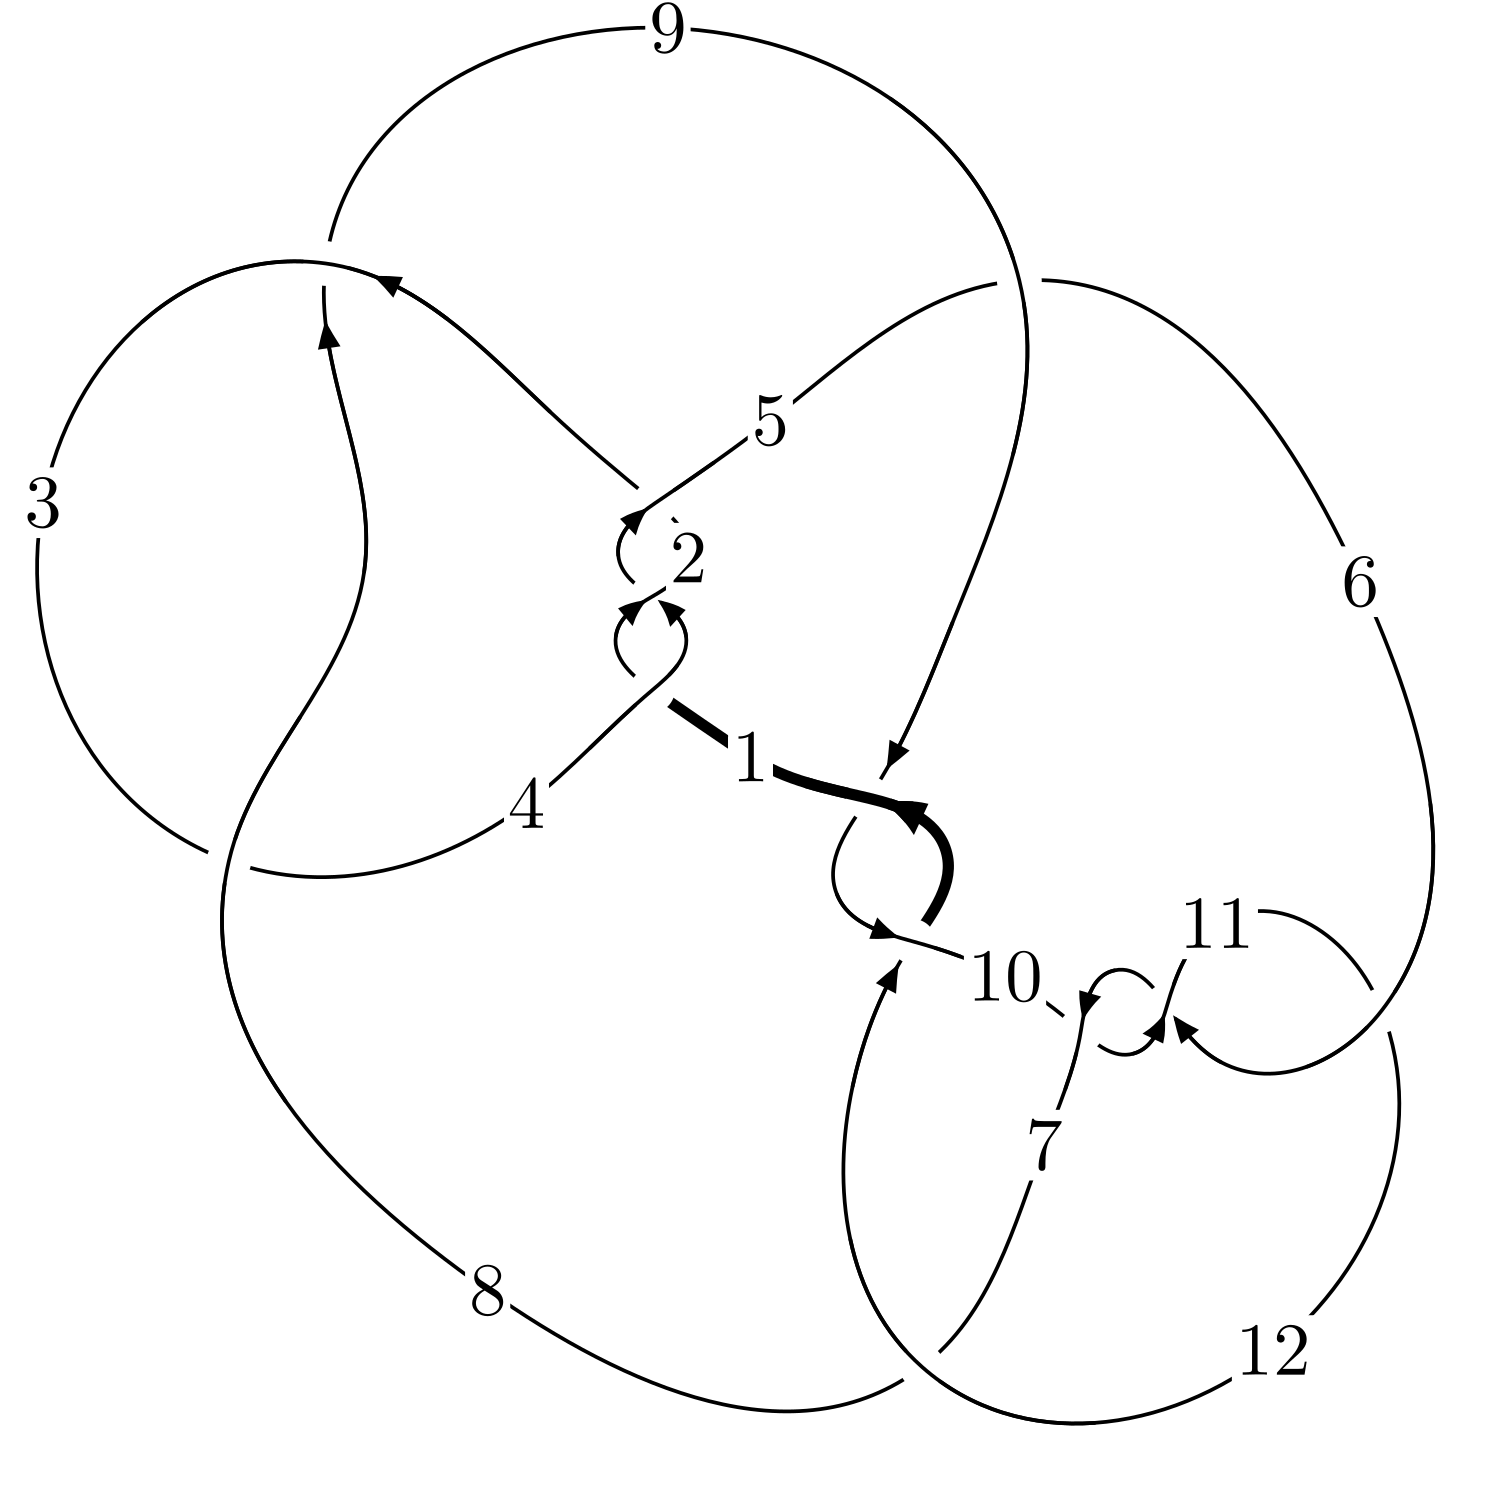
\includegraphics[width=112pt]{../../../GIT/diagram.site/Diagrams/png/1624_12a_0823.png}\\
\ \ \ A knot diagram\footnotemark}&
\allowdisplaybreaks
\textbf{Linearized knot diagam} \\
\cline{2-2}
 &
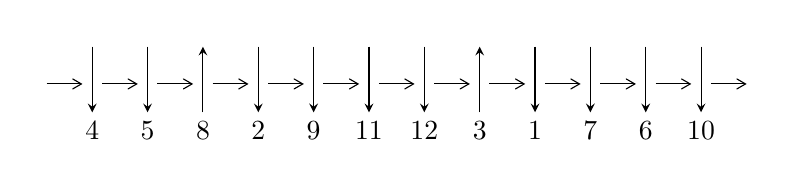
\begin{tikzpicture}[x=20pt, y=17pt]
	% nodes
	\node (C0) at (0, 0) {};
	\node (C1) at (1, 0) {};
	\node (C1U) at (1, +1) {};
	\node (C1D) at (1, -1) {4};

	\node (C2) at (2, 0) {};
	\node (C2U) at (2, +1) {};
	\node (C2D) at (2, -1) {5};

	\node (C3) at (3, 0) {};
	\node (C3U) at (3, +1) {};
	\node (C3D) at (3, -1) {8};

	\node (C4) at (4, 0) {};
	\node (C4U) at (4, +1) {};
	\node (C4D) at (4, -1) {2};

	\node (C5) at (5, 0) {};
	\node (C5U) at (5, +1) {};
	\node (C5D) at (5, -1) {9};

	\node (C6) at (6, 0) {};
	\node (C6U) at (6, +1) {};
	\node (C6D) at (6, -1) {11};

	\node (C7) at (7, 0) {};
	\node (C7U) at (7, +1) {};
	\node (C7D) at (7, -1) {12};

	\node (C8) at (8, 0) {};
	\node (C8U) at (8, +1) {};
	\node (C8D) at (8, -1) {3};

	\node (C9) at (9, 0) {};
	\node (C9U) at (9, +1) {};
	\node (C9D) at (9, -1) {1};

	\node (C10) at (10, 0) {};
	\node (C10U) at (10, +1) {};
	\node (C10D) at (10, -1) {7};

	\node (C11) at (11, 0) {};
	\node (C11U) at (11, +1) {};
	\node (C11D) at (11, -1) {6};

	\node (C12) at (12, 0) {};
	\node (C12U) at (12, +1) {};
	\node (C12D) at (12, -1) {10};
	\node (C13) at (13, 0) {};

	% arrows
	\draw[->,>={angle 60}]
	(C0) edge (C1) (C1) edge (C2) (C2) edge (C3) (C3) edge (C4) (C4) edge (C5) (C5) edge (C6) (C6) edge (C7) (C7) edge (C8) (C8) edge (C9) (C9) edge (C10) (C10) edge (C11) (C11) edge (C12) (C12) edge (C13) ;	\draw[->,>=stealth]
	(C1U) edge (C1D) (C2U) edge (C2D) (C3D) edge (C3U) (C4U) edge (C4D) (C5U) edge (C5D) (C6U) edge (C6D) (C7U) edge (C7D) (C8D) edge (C8U) (C9U) edge (C9D) (C10U) edge (C10D) (C11U) edge (C11D) (C12U) edge (C12D) ;
	\end{tikzpicture} \\
\hhline{~~} \\& 
\textbf{Solving Sequence} \\ \cline{2-2} 
 &
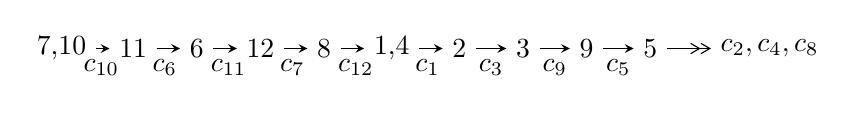
\begin{tikzpicture}[x=23pt, y=7pt]
	% node
	\node (A0) at (-1/8, 0) {7,10};
	\node (A1) at (1, 0) {11};
	\node (A2) at (2, 0) {6};
	\node (A3) at (3, 0) {12};
	\node (A4) at (4, 0) {8};
	\node (A5) at (81/16, 0) {1,4};
	\node (A6) at (49/8, 0) {2};
	\node (A7) at (57/8, 0) {3};
	\node (A8) at (65/8, 0) {9};
	\node (A9) at (73/8, 0) {5};
	\node (C1) at (1/2, -1) {$c_{10}$};
	\node (C2) at (3/2, -1) {$c_{6}$};
	\node (C3) at (5/2, -1) {$c_{11}$};
	\node (C4) at (7/2, -1) {$c_{7}$};
	\node (C5) at (9/2, -1) {$c_{12}$};
	\node (C6) at (45/8, -1) {$c_{1}$};
	\node (C7) at (53/8, -1) {$c_{3}$};
	\node (C8) at (61/8, -1) {$c_{9}$};
	\node (C9) at (69/8, -1) {$c_{5}$};
	\node (A10) at (11, 0) {$c_{2},c_{4},c_{8}$};

	% edge
	\draw[->,>=stealth]	
	(A0) edge (A1) (A1) edge (A2) (A2) edge (A3) (A3) edge (A4) (A4) edge (A5) (A5) edge (A6) (A6) edge (A7) (A7) edge (A8) (A8) edge (A9) ;
	\draw[->>,>={angle 60}]	
	(A9) edge (A10);
\end{tikzpicture} \\ 

\end{tabular} \\

\footnotetext{
The image of knot diagram is generated by the software ``\textbf{Draw programme}" developed by Andrew Bartholomew(\url{http://www.layer8.co.uk/maths/draw/index.htm\#Running-draw}), where we modified some parts for our purpose(\url{https://github.com/CATsTAILs/LinksPainter}).
}\phantom \\ \newline 
\centering \textbf{Ideals for irreducible components\footnotemark of $X_{\text{par}}$} 
 
\begin{align*}
I^u_{1}&=\langle 
2 u^{76}+4 u^{75}+\cdots+b-2,\;-2 u^{75}-2 u^{74}+\cdots+a-5 u,\;u^{77}+2 u^{76}+\cdots-3 u-1\rangle \\
I^u_{2}&=\langle 
b+u,\;a- u+1,\;u^3+2 u+1\rangle \\
I^u_{3}&=\langle 
- u^3+b-2 u+1,\;a-1,\;u^4- u^3+2 u^2-2 u+1\rangle \\
\\
\end{align*}
\raggedright * 3 irreducible components of $\dim_{\mathbb{C}}=0$, with total 84 representations.\\
\footnotetext{All coefficients of polynomials are rational numbers. But the coefficients are sometimes approximated in decimal forms when there is not enough margin.}
\newpage
\renewcommand{\arraystretch}{1}
\centering \section*{I. $I^u_{1}= \langle 2 u^{76}+4 u^{75}+\cdots+b-2,\;-2 u^{75}-2 u^{74}+\cdots+a-5 u,\;u^{77}+2 u^{76}+\cdots-3 u-1 \rangle$}
\flushleft \textbf{(i) Arc colorings}\\
\begin{tabular}{m{7pt} m{180pt} m{7pt} m{180pt} }
\flushright $a_{7}=$&$\begin{pmatrix}0\\u\end{pmatrix}$ \\
\flushright $a_{10}=$&$\begin{pmatrix}1\\0\end{pmatrix}$ \\
\flushright $a_{11}=$&$\begin{pmatrix}1\\u^2\end{pmatrix}$ \\
\flushright $a_{6}=$&$\begin{pmatrix}u\\u^3+u\end{pmatrix}$ \\
\flushright $a_{12}=$&$\begin{pmatrix}u^2+1\\u^4+2 u^2\end{pmatrix}$ \\
\flushright $a_{8}=$&$\begin{pmatrix}- u^5-2 u^3- u\\- u^7-3 u^5-2 u^3+u\end{pmatrix}$ \\
\flushright $a_{1}=$&$\begin{pmatrix}- u^4- u^2+1\\u^4+2 u^2\end{pmatrix}$ \\
\flushright $a_{4}=$&$\begin{pmatrix}2 u^{75}+2 u^{74}+\cdots+10 u^2+5 u\\-2 u^{76}-4 u^{75}+\cdots+4 u+2\end{pmatrix}$ \\
\flushright $a_{2}=$&$\begin{pmatrix}- u^{75}- u^{74}+\cdots-9 u^2-5 u\\u^{76}+2 u^{75}+\cdots- u-1\end{pmatrix}$ \\
\flushright $a_{3}=$&$\begin{pmatrix}u^{71}+u^{70}+\cdots+7 u+1\\- u^{71}-33 u^{69}+\cdots-6 u^2- u\end{pmatrix}$ \\
\flushright $a_{9}=$&$\begin{pmatrix}u^8+3 u^6+u^4-2 u^2+1\\- u^8-4 u^6-4 u^4\end{pmatrix}$ \\
\flushright $a_{5}=$&$\begin{pmatrix}u^{19}+8 u^{17}+24 u^{15}+30 u^{13}+7 u^{11}-10 u^9+4 u^7+6 u^5-3 u^3+2 u\\- u^{19}-9 u^{17}-32 u^{15}-55 u^{13}-43 u^{11}-9 u^9-4 u^5+u^3+u\end{pmatrix}$\\&\end{tabular}
\flushleft \textbf{(ii) Obstruction class $= -1$}\\~\\
\flushleft \textbf{(iii) Cusp Shapes $= 4 u^{76}+8 u^{75}+\cdots-7 u-17$}\\~\\
\newpage\renewcommand{\arraystretch}{1}
\flushleft \textbf{(iv) u-Polynomials at the component}\newline \\
\begin{tabular}{m{50pt}|m{274pt}}
Crossings & \hspace{64pt}u-Polynomials at each crossing \\
\hline $$\begin{aligned}c_{1},c_{2},c_{4}\end{aligned}$$&$\begin{aligned}
&u^{77}-8 u^{76}+\cdots+8 u-1
\end{aligned}$\\
\hline $$\begin{aligned}c_{3},c_{8}\end{aligned}$$&$\begin{aligned}
&u^{77}+u^{76}+\cdots-64 u-128
\end{aligned}$\\
\hline $$\begin{aligned}c_{5}\end{aligned}$$&$\begin{aligned}
&u^{77}+2 u^{76}+\cdots-29557 u-8221
\end{aligned}$\\
\hline $$\begin{aligned}c_{6},c_{10},c_{11}\end{aligned}$$&$\begin{aligned}
&u^{77}+2 u^{76}+\cdots-3 u-1
\end{aligned}$\\
\hline $$\begin{aligned}c_{7}\end{aligned}$$&$\begin{aligned}
&u^{77}-2 u^{76}+\cdots-5736 u-1480
\end{aligned}$\\
\hline $$\begin{aligned}c_{9},c_{12}\end{aligned}$$&$\begin{aligned}
&u^{77}-12 u^{76}+\cdots-1271 u+131
\end{aligned}$\\
\hline
\end{tabular}\\~\\
\newpage\renewcommand{\arraystretch}{1}
\flushleft \textbf{(v) Riley Polynomials at the component}\newline \\
\begin{tabular}{m{50pt}|m{274pt}}
Crossings & \hspace{64pt}Riley Polynomials at each crossing \\
\hline $$\begin{aligned}c_{1},c_{2},c_{4}\end{aligned}$$&$\begin{aligned}
&y^{77}-74 y^{76}+\cdots+40 y-1
\end{aligned}$\\
\hline $$\begin{aligned}c_{3},c_{8}\end{aligned}$$&$\begin{aligned}
&y^{77}+45 y^{76}+\cdots+12288 y-16384
\end{aligned}$\\
\hline $$\begin{aligned}c_{5}\end{aligned}$$&$\begin{aligned}
&y^{77}-24 y^{76}+\cdots+1924884845 y-67584841
\end{aligned}$\\
\hline $$\begin{aligned}c_{6},c_{10},c_{11}\end{aligned}$$&$\begin{aligned}
&y^{77}+72 y^{76}+\cdots+17 y-1
\end{aligned}$\\
\hline $$\begin{aligned}c_{7}\end{aligned}$$&$\begin{aligned}
&y^{77}+24 y^{76}+\cdots-8997104 y-2190400
\end{aligned}$\\
\hline $$\begin{aligned}c_{9},c_{12}\end{aligned}$$&$\begin{aligned}
&y^{77}+60 y^{76}+\cdots+256185 y-17161
\end{aligned}$\\
\hline
\end{tabular}\\~\\
\newpage\flushleft \textbf{(vi) Complex Volumes and Cusp Shapes}
$$\begin{array}{c|c|c}  
\text{Solutions to }I^u_{1}& \I (\text{vol} + \sqrt{-1}CS) & \text{Cusp shape}\\
 \hline 
\begin{aligned}
u &= \phantom{-}0.191592 + 1.136970 I \\
a &= \phantom{-}1.25258 - 0.95288 I \\
b &= \phantom{-}0.250746 + 0.488141 I\end{aligned}
 & -7.29823 + 2.50311 I & \phantom{-0.000000 } 0 \\ \hline\begin{aligned}
u &= \phantom{-}0.191592 - 1.136970 I \\
a &= \phantom{-}1.25258 + 0.95288 I \\
b &= \phantom{-}0.250746 - 0.488141 I\end{aligned}
 & -7.29823 - 2.50311 I & \phantom{-0.000000 } 0 \\ \hline\begin{aligned}
u &= \phantom{-}0.648234 + 0.470762 I \\
a &= \phantom{-}1.50700 - 0.30976 I \\
b &= \phantom{-}0.10743 + 2.01764 I\end{aligned}
 & \phantom{-}0.35199 - 2.14980 I & -12.14186 + 3.38026 I \\ \hline\begin{aligned}
u &= \phantom{-}0.648234 - 0.470762 I \\
a &= \phantom{-}1.50700 + 0.30976 I \\
b &= \phantom{-}0.10743 - 2.01764 I\end{aligned}
 & \phantom{-}0.35199 + 2.14980 I & -12.14186 - 3.38026 I \\ \hline\begin{aligned}
u &= -0.698472 + 0.381933 I \\
a &= \phantom{-}1.38596 - 1.79815 I \\
b &= -2.15973 - 1.56032 I\end{aligned}
 & -5.29571 + 11.59140 I & -11.4531 - 8.4016 I \\ \hline\begin{aligned}
u &= -0.698472 - 0.381933 I \\
a &= \phantom{-}1.38596 + 1.79815 I \\
b &= -2.15973 + 1.56032 I\end{aligned}
 & -5.29571 - 11.59140 I & -11.4531 + 8.4016 I \\ \hline\begin{aligned}
u &= \phantom{-}0.168145 + 1.208940 I \\
a &= -1.04755 + 0.98371 I \\
b &= \phantom{-}0.544196 - 0.621463 I\end{aligned}
 & -0.375128 - 0.568928 I & \phantom{-0.000000 } 0 \\ \hline\begin{aligned}
u &= \phantom{-}0.168145 - 1.208940 I \\
a &= -1.04755 - 0.98371 I \\
b &= \phantom{-}0.544196 + 0.621463 I\end{aligned}
 & -0.375128 + 0.568928 I & \phantom{-0.000000 } 0 \\ \hline\begin{aligned}
u &= -0.543692 + 0.555330 I \\
a &= \phantom{-}0.05223 + 1.78509 I \\
b &= \phantom{-}2.07554 - 1.21742 I\end{aligned}
 & -4.61972 - 7.40639 I & -9.96869 + 2.60400 I \\ \hline\begin{aligned}
u &= -0.543692 - 0.555330 I \\
a &= \phantom{-}0.05223 - 1.78509 I \\
b &= \phantom{-}2.07554 + 1.21742 I\end{aligned}
 & -4.61972 + 7.40639 I & -9.96869 - 2.60400 I\\
 \hline 
 \end{array}$$\newpage$$\begin{array}{c|c|c}  
\text{Solutions to }I^u_{1}& \I (\text{vol} + \sqrt{-1}CS) & \text{Cusp shape}\\
 \hline 
\begin{aligned}
u &= -0.674418 + 0.378910 I \\
a &= -0.51345 + 1.54986 I \\
b &= \phantom{-}2.19270 + 0.48087 I\end{aligned}
 & \phantom{-}0.66148 + 7.43215 I & -8.44278 - 8.42340 I \\ \hline\begin{aligned}
u &= -0.674418 - 0.378910 I \\
a &= -0.51345 - 1.54986 I \\
b &= \phantom{-}2.19270 - 0.48087 I\end{aligned}
 & \phantom{-}0.66148 - 7.43215 I & -8.44278 + 8.42340 I \\ \hline\begin{aligned}
u &= \phantom{-}0.663405 + 0.365765 I \\
a &= -0.41627 - 2.27327 I \\
b &= \phantom{-}1.86641 - 0.34084 I\end{aligned}
 & -2.04586 - 5.11569 I & -10.51933 + 5.70011 I \\ \hline\begin{aligned}
u &= \phantom{-}0.663405 - 0.365765 I \\
a &= -0.41627 + 2.27327 I \\
b &= \phantom{-}1.86641 + 0.34084 I\end{aligned}
 & -2.04586 + 5.11569 I & -10.51933 - 5.70011 I \\ \hline\begin{aligned}
u &= -0.193391 + 1.227550 I \\
a &= -0.055721 - 1.084680 I \\
b &= -1.309470 - 0.174136 I\end{aligned}
 & -2.23828 + 3.03724 I & \phantom{-0.000000 } 0 \\ \hline\begin{aligned}
u &= -0.193391 - 1.227550 I \\
a &= -0.055721 + 1.084680 I \\
b &= -1.309470 + 0.174136 I\end{aligned}
 & -2.23828 - 3.03724 I & \phantom{-0.000000 } 0 \\ \hline\begin{aligned}
u &= \phantom{-}0.636507 + 0.409924 I \\
a &= -0.048390 + 1.303560 I \\
b &= -1.261700 - 0.283097 I\end{aligned}
 & \phantom{-}3.19162 - 3.00945 I & -2.81731 + 4.39327 I \\ \hline\begin{aligned}
u &= \phantom{-}0.636507 - 0.409924 I \\
a &= -0.048390 - 1.303560 I \\
b &= -1.261700 + 0.283097 I\end{aligned}
 & \phantom{-}3.19162 + 3.00945 I & -2.81731 - 4.39327 I \\ \hline\begin{aligned}
u &= \phantom{-}0.581959 + 0.456608 I \\
a &= -0.857892 - 0.656816 I \\
b &= \phantom{-}1.210810 - 0.588589 I\end{aligned}
 & \phantom{-}3.40919 - 0.96956 I & -2.16570 + 2.84354 I \\ \hline\begin{aligned}
u &= \phantom{-}0.581959 - 0.456608 I \\
a &= -0.857892 + 0.656816 I \\
b &= \phantom{-}1.210810 + 0.588589 I\end{aligned}
 & \phantom{-}3.40919 + 0.96956 I & -2.16570 - 2.84354 I\\
 \hline 
 \end{array}$$\newpage$$\begin{array}{c|c|c}  
\text{Solutions to }I^u_{1}& \I (\text{vol} + \sqrt{-1}CS) & \text{Cusp shape}\\
 \hline 
\begin{aligned}
u &= -0.530488 + 0.512932 I \\
a &= \phantom{-}0.53897 - 1.77641 I \\
b &= -1.88073 + 0.09967 I\end{aligned}
 & \phantom{-}1.24122 - 3.41237 I & -6.71316 + 2.36836 I \\ \hline\begin{aligned}
u &= -0.530488 - 0.512932 I \\
a &= \phantom{-}0.53897 + 1.77641 I \\
b &= -1.88073 - 0.09967 I\end{aligned}
 & \phantom{-}1.24122 + 3.41237 I & -6.71316 - 2.36836 I \\ \hline\begin{aligned}
u &= \phantom{-}0.205270 + 1.249720 I \\
a &= \phantom{-}0.558990 - 0.770110 I \\
b &= -0.751957 + 1.042090 I\end{aligned}
 & \phantom{-}0.05560 - 5.43305 I & \phantom{-0.000000 } 0 \\ \hline\begin{aligned}
u &= \phantom{-}0.205270 - 1.249720 I \\
a &= \phantom{-}0.558990 + 0.770110 I \\
b &= -0.751957 - 1.042090 I\end{aligned}
 & \phantom{-}0.05560 + 5.43305 I & \phantom{-0.000000 } 0 \\ \hline\begin{aligned}
u &= -0.639232 + 0.359723 I \\
a &= -0.341288 - 0.577957 I \\
b &= -1.35130 + 0.64186 I\end{aligned}
 & -0.67724 + 2.50744 I & -11.34570 - 3.59018 I \\ \hline\begin{aligned}
u &= -0.639232 - 0.359723 I \\
a &= -0.341288 + 0.577957 I \\
b &= -1.35130 - 0.64186 I\end{aligned}
 & -0.67724 - 2.50744 I & -11.34570 + 3.59018 I \\ \hline\begin{aligned}
u &= -0.665128 + 0.278108 I \\
a &= -0.319540 - 0.999371 I \\
b &= -0.008826 - 0.427772 I\end{aligned}
 & -8.17542 + 0.47611 I & -14.7158 - 2.7445 I \\ \hline\begin{aligned}
u &= -0.665128 - 0.278108 I \\
a &= -0.319540 + 0.999371 I \\
b &= -0.008826 + 0.427772 I\end{aligned}
 & -8.17542 - 0.47611 I & -14.7158 + 2.7445 I \\ \hline\begin{aligned}
u &= \phantom{-}0.244033 + 1.257390 I \\
a &= -0.490522 + 0.142450 I \\
b &= \phantom{-}0.92817 - 1.27652 I\end{aligned}
 & -6.42273 - 9.14754 I & \phantom{-0.000000 } 0 \\ \hline\begin{aligned}
u &= \phantom{-}0.244033 - 1.257390 I \\
a &= -0.490522 - 0.142450 I \\
b &= \phantom{-}0.92817 + 1.27652 I\end{aligned}
 & -6.42273 + 9.14754 I & \phantom{-0.000000 } 0\\
 \hline 
 \end{array}$$\newpage$$\begin{array}{c|c|c}  
\text{Solutions to }I^u_{1}& \I (\text{vol} + \sqrt{-1}CS) & \text{Cusp shape}\\
 \hline 
\begin{aligned}
u &= -0.140039 + 1.287520 I \\
a &= \phantom{-}0.024976 + 0.385611 I \\
b &= \phantom{-}0.504759 - 0.003724 I\end{aligned}
 & \phantom{-}3.01135 + 2.29522 I & \phantom{-0.000000 } 0 \\ \hline\begin{aligned}
u &= -0.140039 - 1.287520 I \\
a &= \phantom{-}0.024976 - 0.385611 I \\
b &= \phantom{-}0.504759 + 0.003724 I\end{aligned}
 & \phantom{-}3.01135 - 2.29522 I & \phantom{-0.000000 } 0 \\ \hline\begin{aligned}
u &= \phantom{-}0.501793 + 0.490701 I \\
a &= \phantom{-}0.860902 + 0.742398 I \\
b &= -1.82723 - 0.06586 I\end{aligned}
 & -1.44185 + 1.23982 I & -8.66150 + 0.75675 I \\ \hline\begin{aligned}
u &= \phantom{-}0.501793 - 0.490701 I \\
a &= \phantom{-}0.860902 - 0.742398 I \\
b &= -1.82723 + 0.06586 I\end{aligned}
 & -1.44185 - 1.23982 I & -8.66150 - 0.75675 I \\ \hline\begin{aligned}
u &= \phantom{-}0.030612 + 1.300700 I \\
a &= -1.43632 - 0.09108 I \\
b &= \phantom{-}0.806088 + 1.056020 I\end{aligned}
 & \phantom{-}1.81589 - 0.96118 I & \phantom{-0.000000 } 0 \\ \hline\begin{aligned}
u &= \phantom{-}0.030612 - 1.300700 I \\
a &= -1.43632 + 0.09108 I \\
b &= \phantom{-}0.806088 - 1.056020 I\end{aligned}
 & \phantom{-}1.81589 + 0.96118 I & \phantom{-0.000000 } 0 \\ \hline\begin{aligned}
u &= -0.317735 + 0.605450 I \\
a &= \phantom{-}0.780897 - 0.702370 I \\
b &= \phantom{-}0.427338 - 0.189042 I\end{aligned}
 & -6.84784 + 3.07044 I & -11.28075 - 3.47607 I \\ \hline\begin{aligned}
u &= -0.317735 - 0.605450 I \\
a &= \phantom{-}0.780897 + 0.702370 I \\
b &= \phantom{-}0.427338 + 0.189042 I\end{aligned}
 & -6.84784 - 3.07044 I & -11.28075 + 3.47607 I \\ \hline\begin{aligned}
u &= \phantom{-}0.677966 + 0.062750 I \\
a &= -1.315350 + 0.451550 I \\
b &= -0.615406 + 0.909035 I\end{aligned}
 & -10.48850 - 5.79061 I & -17.0367 + 4.4441 I \\ \hline\begin{aligned}
u &= \phantom{-}0.677966 - 0.062750 I \\
a &= -1.315350 - 0.451550 I \\
b &= -0.615406 - 0.909035 I\end{aligned}
 & -10.48850 + 5.79061 I & -17.0367 - 4.4441 I\\
 \hline 
 \end{array}$$\newpage$$\begin{array}{c|c|c}  
\text{Solutions to }I^u_{1}& \I (\text{vol} + \sqrt{-1}CS) & \text{Cusp shape}\\
 \hline 
\begin{aligned}
u &= -0.508655 + 0.424322 I \\
a &= -1.11823 + 1.18156 I \\
b &= \phantom{-}0.738302 + 1.005860 I\end{aligned}
 & -0.212543 + 1.167780 I & -10.21646 - 3.31814 I \\ \hline\begin{aligned}
u &= -0.508655 - 0.424322 I \\
a &= -1.11823 - 1.18156 I \\
b &= \phantom{-}0.738302 - 1.005860 I\end{aligned}
 & -0.212543 - 1.167780 I & -10.21646 + 3.31814 I \\ \hline\begin{aligned}
u &= -0.046345 + 1.356970 I \\
a &= \phantom{-}0.429786 + 0.365022 I \\
b &= \phantom{-}0.054673 - 0.996286 I\end{aligned}
 & \phantom{-}4.57102 + 1.91273 I & \phantom{-0.000000 } 0 \\ \hline\begin{aligned}
u &= -0.046345 - 1.356970 I \\
a &= \phantom{-}0.429786 - 0.365022 I \\
b &= \phantom{-}0.054673 + 0.996286 I\end{aligned}
 & \phantom{-}4.57102 - 1.91273 I & \phantom{-0.000000 } 0 \\ \hline\begin{aligned}
u &= -0.634684\phantom{ +0.000000I} \\
a &= \phantom{-}2.01220\phantom{ +0.000000I} \\
b &= \phantom{-}1.27931\phantom{ +0.000000I}\end{aligned}
 & -5.94766\phantom{ +0.000000I} & -16.5240\phantom{ +0.000000I} \\ \hline\begin{aligned}
u &= \phantom{-}0.630519 + 0.033395 I \\
a &= \phantom{-}0.592203 + 0.279484 I \\
b &= \phantom{-}0.148921 - 0.802727 I\end{aligned}
 & -3.86408 - 2.37823 I & -15.7846 + 4.2598 I \\ \hline\begin{aligned}
u &= \phantom{-}0.630519 - 0.033395 I \\
a &= \phantom{-}0.592203 - 0.279484 I \\
b &= \phantom{-}0.148921 + 0.802727 I\end{aligned}
 & -3.86408 + 2.37823 I & -15.7846 - 4.2598 I \\ \hline\begin{aligned}
u &= -0.25087 + 1.40762 I \\
a &= \phantom{-}0.0478365 + 0.1135190 I \\
b &= -0.127222 + 0.654262 I\end{aligned}
 & -2.79475 + 3.80266 I & \phantom{-0.000000 } 0 \\ \hline\begin{aligned}
u &= -0.25087 - 1.40762 I \\
a &= \phantom{-}0.0478365 - 0.1135190 I \\
b &= -0.127222 - 0.654262 I\end{aligned}
 & -2.79475 - 3.80266 I & \phantom{-0.000000 } 0 \\ \hline\begin{aligned}
u &= -0.07700 + 1.42792 I \\
a &= \phantom{-}0.476070 - 0.097068 I \\
b &= -1.006700 + 0.604162 I\end{aligned}
 & -0.55532 + 4.30754 I & \phantom{-0.000000 } 0\\
 \hline 
 \end{array}$$\newpage$$\begin{array}{c|c|c}  
\text{Solutions to }I^u_{1}& \I (\text{vol} + \sqrt{-1}CS) & \text{Cusp shape}\\
 \hline 
\begin{aligned}
u &= -0.07700 - 1.42792 I \\
a &= \phantom{-}0.476070 + 0.097068 I \\
b &= -1.006700 - 0.604162 I\end{aligned}
 & -0.55532 - 4.30754 I & \phantom{-0.000000 } 0 \\ \hline\begin{aligned}
u &= -0.20019 + 1.44614 I \\
a &= \phantom{-}2.10795 + 0.53113 I \\
b &= -0.92627 - 1.55636 I\end{aligned}
 & \phantom{-}5.75987 + 3.83600 I & \phantom{-0.000000 } 0 \\ \hline\begin{aligned}
u &= -0.20019 - 1.44614 I \\
a &= \phantom{-}2.10795 - 0.53113 I \\
b &= -0.92627 + 1.55636 I\end{aligned}
 & \phantom{-}5.75987 - 3.83600 I & \phantom{-0.000000 } 0 \\ \hline\begin{aligned}
u &= -0.24286 + 1.44306 I \\
a &= -1.29039 + 1.70660 I \\
b &= \phantom{-}1.72235 - 0.79745 I\end{aligned}
 & \phantom{-}5.11778 + 5.74279 I & \phantom{-0.000000 } 0 \\ \hline\begin{aligned}
u &= -0.24286 - 1.44306 I \\
a &= -1.29039 - 1.70660 I \\
b &= \phantom{-}1.72235 + 0.79745 I\end{aligned}
 & \phantom{-}5.11778 - 5.74279 I & \phantom{-0.000000 } 0 \\ \hline\begin{aligned}
u &= \phantom{-}0.18621 + 1.45304 I \\
a &= -2.92205 - 0.73186 I \\
b &= \phantom{-}2.10609 - 0.10486 I\end{aligned}
 & \phantom{-}4.73087 - 1.28332 I & \phantom{-0.000000 } 0 \\ \hline\begin{aligned}
u &= \phantom{-}0.18621 - 1.45304 I \\
a &= -2.92205 + 0.73186 I \\
b &= \phantom{-}2.10609 + 0.10486 I\end{aligned}
 & \phantom{-}4.73087 + 1.28332 I & \phantom{-0.000000 } 0 \\ \hline\begin{aligned}
u &= \phantom{-}0.25081 + 1.44678 I \\
a &= \phantom{-}2.48049 + 1.77440 I \\
b &= -1.99607 + 0.46680 I\end{aligned}
 & \phantom{-}3.78033 - 8.45891 I & \phantom{-0.000000 } 0 \\ \hline\begin{aligned}
u &= \phantom{-}0.25081 - 1.44678 I \\
a &= \phantom{-}2.48049 - 1.77440 I \\
b &= -1.99607 - 0.46680 I\end{aligned}
 & \phantom{-}3.78033 + 8.45891 I & \phantom{-0.000000 } 0 \\ \hline\begin{aligned}
u &= -0.25374 + 1.45283 I \\
a &= \phantom{-}2.99683 - 1.30974 I \\
b &= -2.52211 - 0.52460 I\end{aligned}
 & \phantom{-}6.55336 + 10.82390 I & \phantom{-0.000000 } 0\\
 \hline 
 \end{array}$$\newpage$$\begin{array}{c|c|c}  
\text{Solutions to }I^u_{1}& \I (\text{vol} + \sqrt{-1}CS) & \text{Cusp shape}\\
 \hline 
\begin{aligned}
u &= -0.25374 - 1.45283 I \\
a &= \phantom{-}2.99683 + 1.30974 I \\
b &= -2.52211 + 0.52460 I\end{aligned}
 & \phantom{-}6.55336 - 10.82390 I & \phantom{-0.000000 } 0 \\ \hline\begin{aligned}
u &= -0.18475 + 1.46518 I \\
a &= -2.66257 + 1.18028 I \\
b &= \phantom{-}2.11134 + 0.37230 I\end{aligned}
 & \phantom{-}7.57007 - 0.82609 I & \phantom{-0.000000 } 0 \\ \hline\begin{aligned}
u &= -0.18475 - 1.46518 I \\
a &= -2.66257 - 1.18028 I \\
b &= \phantom{-}2.11134 - 0.37230 I\end{aligned}
 & \phantom{-}7.57007 + 0.82609 I & \phantom{-0.000000 } 0 \\ \hline\begin{aligned}
u &= \phantom{-}0.23586 + 1.45906 I \\
a &= -1.42551 - 1.47383 I \\
b &= \phantom{-}1.45011 + 0.16039 I\end{aligned}
 & \phantom{-}9.20898 - 6.20501 I & \phantom{-0.000000 } 0 \\ \hline\begin{aligned}
u &= \phantom{-}0.23586 - 1.45906 I \\
a &= -1.42551 + 1.47383 I \\
b &= \phantom{-}1.45011 - 0.16039 I\end{aligned}
 & \phantom{-}9.20898 + 6.20501 I & \phantom{-0.000000 } 0 \\ \hline\begin{aligned}
u &= \phantom{-}0.21070 + 1.46383 I \\
a &= \phantom{-}2.24094 - 0.01125 I \\
b &= -1.43080 + 0.77753 I\end{aligned}
 & \phantom{-}9.58297 - 3.87222 I & \phantom{-0.000000 } 0 \\ \hline\begin{aligned}
u &= \phantom{-}0.21070 - 1.46383 I \\
a &= \phantom{-}2.24094 + 0.01125 I \\
b &= -1.43080 - 0.77753 I\end{aligned}
 & \phantom{-}9.58297 + 3.87222 I & \phantom{-0.000000 } 0 \\ \hline\begin{aligned}
u &= -0.26298 + 1.45689 I \\
a &= -3.77652 + 0.35669 I \\
b &= \phantom{-}2.35692 + 1.70683 I\end{aligned}
 & \phantom{-}0.6203 + 15.0997 I & \phantom{-0.000000 } 0 \\ \hline\begin{aligned}
u &= -0.26298 - 1.45689 I \\
a &= -3.77652 - 0.35669 I \\
b &= \phantom{-}2.35692 - 1.70683 I\end{aligned}
 & \phantom{-}0.6203 - 15.0997 I & \phantom{-0.000000 } 0 \\ \hline\begin{aligned}
u &= -0.17434 + 1.47906 I \\
a &= \phantom{-}2.32909 - 2.44851 I \\
b &= -2.38054 + 0.94253 I\end{aligned}
 & \phantom{-}1.93159 - 4.85744 I & \phantom{-0.000000 } 0\\
 \hline 
 \end{array}$$\newpage$$\begin{array}{c|c|c}  
\text{Solutions to }I^u_{1}& \I (\text{vol} + \sqrt{-1}CS) & \text{Cusp shape}\\
 \hline 
\begin{aligned}
u &= -0.17434 - 1.47906 I \\
a &= \phantom{-}2.32909 + 2.44851 I \\
b &= -2.38054 - 0.94253 I\end{aligned}
 & \phantom{-}1.93159 + 4.85744 I & \phantom{-0.000000 } 0 \\ \hline\begin{aligned}
u &= -0.500819\phantom{ +0.000000I} \\
a &= -0.741044\phantom{ +0.000000I} \\
b &= -0.370645\phantom{ +0.000000I}\end{aligned}
 & -0.969871\phantom{ +0.000000I} & -9.81070\phantom{ +0.000000I} \\ \hline\begin{aligned}
u &= \phantom{-}0.22825 + 1.48172 I \\
a &= -1.26848 + 2.30843 I \\
b &= -0.22862 - 2.16336 I\end{aligned}
 & \phantom{-}6.66843 - 5.34198 I & \phantom{-0.000000 } 0 \\ \hline\begin{aligned}
u &= \phantom{-}0.22825 - 1.48172 I \\
a &= -1.26848 - 2.30843 I \\
b &= -0.22862 + 2.16336 I\end{aligned}
 & \phantom{-}6.66843 + 5.34198 I & \phantom{-0.000000 } 0 \\ \hline\begin{aligned}
u &= -0.258129 + 0.312221 I \\
a &= -0.91822 + 1.08073 I \\
b &= \phantom{-}0.070880 + 0.493977 I\end{aligned}
 & -0.483753 + 0.975967 I & -7.83160 - 6.63357 I \\ \hline\begin{aligned}
u &= -0.258129 - 0.312221 I \\
a &= -0.91822 - 1.08073 I \\
b &= \phantom{-}0.070880 - 0.493977 I\end{aligned}
 & -0.483753 - 0.975967 I & -7.83160 + 6.63357 I \\ \hline\begin{aligned}
u &= \phantom{-}0.276652\phantom{ +0.000000I} \\
a &= \phantom{-}2.84998\phantom{ +0.000000I} \\
b &= -0.686858\phantom{ +0.000000I}\end{aligned}
 & -2.04721\phantom{ +0.000000I} & \phantom{-}0.166320\phantom{ +0.000000I}\\
 \hline 
 \end{array}$$\newpage\newpage\renewcommand{\arraystretch}{1}
\centering \section*{II. $I^u_{2}= \langle b+u,\;a- u+1,\;u^3+2 u+1 \rangle$}
\flushleft \textbf{(i) Arc colorings}\\
\begin{tabular}{m{7pt} m{180pt} m{7pt} m{180pt} }
\flushright $a_{7}=$&$\begin{pmatrix}0\\u\end{pmatrix}$ \\
\flushright $a_{10}=$&$\begin{pmatrix}1\\0\end{pmatrix}$ \\
\flushright $a_{11}=$&$\begin{pmatrix}1\\u^2\end{pmatrix}$ \\
\flushright $a_{6}=$&$\begin{pmatrix}u\\- u-1\end{pmatrix}$ \\
\flushright $a_{12}=$&$\begin{pmatrix}u^2+1\\- u\end{pmatrix}$ \\
\flushright $a_{8}=$&$\begin{pmatrix}u^2- u\\- u^2\end{pmatrix}$ \\
\flushright $a_{1}=$&$\begin{pmatrix}u^2+u+1\\- u\end{pmatrix}$ \\
\flushright $a_{4}=$&$\begin{pmatrix}u-1\\- u\end{pmatrix}$ \\
\flushright $a_{2}=$&$\begin{pmatrix}u^2+2 u\\-2 u\end{pmatrix}$ \\
\flushright $a_{3}=$&$\begin{pmatrix}u-1\\- u\end{pmatrix}$ \\
\flushright $a_{9}=$&$\begin{pmatrix}u^2- u\\- u^2\end{pmatrix}$ \\
\flushright $a_{5}=$&$\begin{pmatrix}- u^2- u-1\\u\end{pmatrix}$\\&\end{tabular}
\flushleft \textbf{(ii) Obstruction class $= 1$}\\~\\
\flushleft \textbf{(iii) Cusp Shapes $= -7 u^2+5 u-18$}\\~\\
\newpage\renewcommand{\arraystretch}{1}
\flushleft \textbf{(iv) u-Polynomials at the component}\newline \\
\begin{tabular}{m{50pt}|m{274pt}}
Crossings & \hspace{64pt}u-Polynomials at each crossing \\
\hline $$\begin{aligned}c_{1},c_{2}\end{aligned}$$&$\begin{aligned}
&(u-1)^3
\end{aligned}$\\
\hline $$\begin{aligned}c_{3},c_{8}\end{aligned}$$&$\begin{aligned}
&u^3
\end{aligned}$\\
\hline $$\begin{aligned}c_{4}\end{aligned}$$&$\begin{aligned}
&(u+1)^3
\end{aligned}$\\
\hline $$\begin{aligned}c_{5},c_{6},c_{9}\end{aligned}$$&$\begin{aligned}
&u^3+2 u-1
\end{aligned}$\\
\hline $$\begin{aligned}c_{7}\end{aligned}$$&$\begin{aligned}
&u^3-3 u^2+5 u-2
\end{aligned}$\\
\hline $$\begin{aligned}c_{10},c_{11},c_{12}\end{aligned}$$&$\begin{aligned}
&u^3+2 u+1
\end{aligned}$\\
\hline
\end{tabular}\\~\\
\newpage\renewcommand{\arraystretch}{1}
\flushleft \textbf{(v) Riley Polynomials at the component}\newline \\
\begin{tabular}{m{50pt}|m{274pt}}
Crossings & \hspace{64pt}Riley Polynomials at each crossing \\
\hline $$\begin{aligned}c_{1},c_{2},c_{4}\end{aligned}$$&$\begin{aligned}
&(y-1)^3
\end{aligned}$\\
\hline $$\begin{aligned}c_{3},c_{8}\end{aligned}$$&$\begin{aligned}
&y^3
\end{aligned}$\\
\hline $$\begin{aligned}c_{5},c_{6},c_{9}\\c_{10},c_{11},c_{12}\end{aligned}$$&$\begin{aligned}
&y^3+4 y^2+4 y-1
\end{aligned}$\\
\hline $$\begin{aligned}c_{7}\end{aligned}$$&$\begin{aligned}
&y^3+y^2+13 y-4
\end{aligned}$\\
\hline
\end{tabular}\\~\\
\newpage\flushleft \textbf{(vi) Complex Volumes and Cusp Shapes}
$$\begin{array}{c|c|c}  
\text{Solutions to }I^u_{2}& \I (\text{vol} + \sqrt{-1}CS) & \text{Cusp shape}\\
 \hline 
\begin{aligned}
u &= \phantom{-}0.22670 + 1.46771 I \\
a &= -0.77330 + 1.46771 I \\
b &= -0.22670 - 1.46771 I\end{aligned}
 & \phantom{-}7.79580 - 5.13794 I & -2.14701 + 2.68036 I \\ \hline\begin{aligned}
u &= \phantom{-}0.22670 - 1.46771 I \\
a &= -0.77330 - 1.46771 I \\
b &= -0.22670 + 1.46771 I\end{aligned}
 & \phantom{-}7.79580 + 5.13794 I & -2.14701 - 2.68036 I \\ \hline\begin{aligned}
u &= -0.453398\phantom{ +0.000000I} \\
a &= -1.45340\phantom{ +0.000000I} \\
b &= \phantom{-}0.453398\phantom{ +0.000000I}\end{aligned}
 & -2.43213\phantom{ +0.000000I} & -21.7060\phantom{ +0.000000I}\\
 \hline 
 \end{array}$$\newpage\newpage\renewcommand{\arraystretch}{1}
\centering \section*{III. $I^u_{3}= \langle - u^3+b-2 u+1,\;a-1,\;u^4- u^3+2 u^2-2 u+1 \rangle$}
\flushleft \textbf{(i) Arc colorings}\\
\begin{tabular}{m{7pt} m{180pt} m{7pt} m{180pt} }
\flushright $a_{7}=$&$\begin{pmatrix}0\\u\end{pmatrix}$ \\
\flushright $a_{10}=$&$\begin{pmatrix}1\\0\end{pmatrix}$ \\
\flushright $a_{11}=$&$\begin{pmatrix}1\\u^2\end{pmatrix}$ \\
\flushright $a_{6}=$&$\begin{pmatrix}u\\u^3+u\end{pmatrix}$ \\
\flushright $a_{12}=$&$\begin{pmatrix}u^2+1\\u^3+2 u-1\end{pmatrix}$ \\
\flushright $a_{8}=$&$\begin{pmatrix}- u^3-2 u+1\\- u^3+u^2- u+2\end{pmatrix}$ \\
\flushright $a_{1}=$&$\begin{pmatrix}- u^3+u^2-2 u+2\\u^3+2 u-1\end{pmatrix}$ \\
\flushright $a_{4}=$&$\begin{pmatrix}1\\u^3+2 u-1\end{pmatrix}$ \\
\flushright $a_{2}=$&$\begin{pmatrix}- u^3+u^2-2 u+3\\2 u^3+4 u-2\end{pmatrix}$ \\
\flushright $a_{3}=$&$\begin{pmatrix}1\\u^3+2 u-1\end{pmatrix}$ \\
\flushright $a_{9}=$&$\begin{pmatrix}- u^3-2 u+1\\- u^3+u^2- u+2\end{pmatrix}$ \\
\flushright $a_{5}=$&$\begin{pmatrix}u^3- u^2+2 u-2\\- u^3-2 u+1\end{pmatrix}$\\&\end{tabular}
\flushleft \textbf{(ii) Obstruction class $= 1$}\\~\\
\flushleft \textbf{(iii) Cusp Shapes $= 3 u^3+2 u^2+2 u-7$}\\~\\
\newpage\renewcommand{\arraystretch}{1}
\flushleft \textbf{(iv) u-Polynomials at the component}\newline \\
\begin{tabular}{m{50pt}|m{274pt}}
Crossings & \hspace{64pt}u-Polynomials at each crossing \\
\hline $$\begin{aligned}c_{1},c_{2}\end{aligned}$$&$\begin{aligned}
&(u-1)^4
\end{aligned}$\\
\hline $$\begin{aligned}c_{3},c_{8}\end{aligned}$$&$\begin{aligned}
&u^4
\end{aligned}$\\
\hline $$\begin{aligned}c_{4}\end{aligned}$$&$\begin{aligned}
&(u+1)^4
\end{aligned}$\\
\hline $$\begin{aligned}c_{5},c_{6},c_{9}\end{aligned}$$&$\begin{aligned}
&u^4+u^3+2 u^2+2 u+1
\end{aligned}$\\
\hline $$\begin{aligned}c_{7}\end{aligned}$$&$\begin{aligned}
&(u^2+u+1)^2
\end{aligned}$\\
\hline $$\begin{aligned}c_{10},c_{11},c_{12}\end{aligned}$$&$\begin{aligned}
&u^4- u^3+2 u^2-2 u+1
\end{aligned}$\\
\hline
\end{tabular}\\~\\
\newpage\renewcommand{\arraystretch}{1}
\flushleft \textbf{(v) Riley Polynomials at the component}\newline \\
\begin{tabular}{m{50pt}|m{274pt}}
Crossings & \hspace{64pt}Riley Polynomials at each crossing \\
\hline $$\begin{aligned}c_{1},c_{2},c_{4}\end{aligned}$$&$\begin{aligned}
&(y-1)^4
\end{aligned}$\\
\hline $$\begin{aligned}c_{3},c_{8}\end{aligned}$$&$\begin{aligned}
&y^4
\end{aligned}$\\
\hline $$\begin{aligned}c_{5},c_{6},c_{9}\\c_{10},c_{11},c_{12}\end{aligned}$$&$\begin{aligned}
&y^4+3 y^3+2 y^2+1
\end{aligned}$\\
\hline $$\begin{aligned}c_{7}\end{aligned}$$&$\begin{aligned}
&(y^2+y+1)^2
\end{aligned}$\\
\hline
\end{tabular}\\~\\
\newpage\flushleft \textbf{(vi) Complex Volumes and Cusp Shapes}
$$\begin{array}{c|c|c}  
\text{Solutions to }I^u_{3}& \I (\text{vol} + \sqrt{-1}CS) & \text{Cusp shape}\\
 \hline 
\begin{aligned}
u &= \phantom{-}0.621744 + 0.440597 I \\
a &= \phantom{-}1.00000\phantom{ +0.000000I} \\
b &= \phantom{-}0.121744 + 1.306620 I\end{aligned}
 & \phantom{-}1.64493 - 2.02988 I & -5.73686 + 3.25323 I \\ \hline\begin{aligned}
u &= \phantom{-}0.621744 - 0.440597 I \\
a &= \phantom{-}1.00000\phantom{ +0.000000I} \\
b &= \phantom{-}0.121744 - 1.306620 I\end{aligned}
 & \phantom{-}1.64493 + 2.02988 I & -5.73686 - 3.25323 I \\ \hline\begin{aligned}
u &= -0.121744 + 1.306620 I \\
a &= \phantom{-}1.00000\phantom{ +0.000000I} \\
b &= -0.621744 + 0.440597 I\end{aligned}
 & \phantom{-}1.64493 + 2.02988 I & -8.76314 - 4.54099 I \\ \hline\begin{aligned}
u &= -0.121744 - 1.306620 I \\
a &= \phantom{-}1.00000\phantom{ +0.000000I} \\
b &= -0.621744 - 0.440597 I\end{aligned}
 & \phantom{-}1.64493 - 2.02988 I & -8.76314 + 4.54099 I\\
 \hline 
 \end{array}$$\newpage
\newpage\renewcommand{\arraystretch}{1}
\centering \section*{ IV. u-Polynomials}
\begin{tabular}{m{50pt}|m{274pt}}
Crossings & \hspace{64pt}u-Polynomials at each crossing \\
\hline $$\begin{aligned}c_{1},c_{2}\end{aligned}$$&$\begin{aligned}
&((u-1)^7)(u^{77}-8 u^{76}+\cdots+8 u-1)
\end{aligned}$\\
\hline $$\begin{aligned}c_{3},c_{8}\end{aligned}$$&$\begin{aligned}
&u^7(u^{77}+u^{76}+\cdots-64 u-128)
\end{aligned}$\\
\hline $$\begin{aligned}c_{4}\end{aligned}$$&$\begin{aligned}
&((u+1)^7)(u^{77}-8 u^{76}+\cdots+8 u-1)
\end{aligned}$\\
\hline $$\begin{aligned}c_{5}\end{aligned}$$&$\begin{aligned}
&(u^3+2 u-1)(u^4+u^3+2 u^2+2 u+1)(u^{77}+2 u^{76}+\cdots-29557 u-8221)
\end{aligned}$\\
\hline $$\begin{aligned}c_{6}\end{aligned}$$&$\begin{aligned}
&(u^3+2 u-1)(u^4+u^3+2 u^2+2 u+1)(u^{77}+2 u^{76}+\cdots-3 u-1)
\end{aligned}$\\
\hline $$\begin{aligned}c_{7}\end{aligned}$$&$\begin{aligned}
&((u^2+u+1)^2)(u^3-3 u^2+5 u-2)(u^{77}-2 u^{76}+\cdots-5736 u-1480)
\end{aligned}$\\
\hline $$\begin{aligned}c_{9}\end{aligned}$$&$\begin{aligned}
&(u^3+2 u-1)(u^4+u^3+2 u^2+2 u+1)(u^{77}-12 u^{76}+\cdots-1271 u+131)
\end{aligned}$\\
\hline $$\begin{aligned}c_{10},c_{11}\end{aligned}$$&$\begin{aligned}
&(u^3+2 u+1)(u^4- u^3+2 u^2-2 u+1)(u^{77}+2 u^{76}+\cdots-3 u-1)
\end{aligned}$\\
\hline $$\begin{aligned}c_{12}\end{aligned}$$&$\begin{aligned}
&(u^3+2 u+1)(u^4- u^3+2 u^2-2 u+1)(u^{77}-12 u^{76}+\cdots-1271 u+131)
\end{aligned}$\\
\hline
\end{tabular}\newpage\renewcommand{\arraystretch}{1}
\centering \section*{ V. Riley Polynomials}
\begin{tabular}{m{50pt}|m{274pt}}
Crossings & \hspace{64pt}Riley Polynomials at each crossing \\
\hline $$\begin{aligned}c_{1},c_{2},c_{4}\end{aligned}$$&$\begin{aligned}
&((y-1)^7)(y^{77}-74 y^{76}+\cdots+40 y-1)
\end{aligned}$\\
\hline $$\begin{aligned}c_{3},c_{8}\end{aligned}$$&$\begin{aligned}
&y^7(y^{77}+45 y^{76}+\cdots+12288 y-16384)
\end{aligned}$\\
\hline $$\begin{aligned}c_{5}\end{aligned}$$&$\begin{aligned}
&(y^3+4 y^2+4 y-1)(y^4+3 y^3+2 y^2+1)\\
&\cdot(y^{77}-24 y^{76}+\cdots+1924884845 y-67584841)
\end{aligned}$\\
\hline $$\begin{aligned}c_{6},c_{10},c_{11}\end{aligned}$$&$\begin{aligned}
&(y^3+4 y^2+4 y-1)(y^4+3 y^3+2 y^2+1)(y^{77}+72 y^{76}+\cdots+17 y-1)
\end{aligned}$\\
\hline $$\begin{aligned}c_{7}\end{aligned}$$&$\begin{aligned}
&(y^2+y+1)^2(y^3+y^2+13 y-4)\\
&\cdot(y^{77}+24 y^{76}+\cdots-8997104 y-2190400)
\end{aligned}$\\
\hline $$\begin{aligned}c_{9},c_{12}\end{aligned}$$&$\begin{aligned}
&(y^3+4 y^2+4 y-1)(y^4+3 y^3+2 y^2+1)\\
&\cdot(y^{77}+60 y^{76}+\cdots+256185 y-17161)
\end{aligned}$\\
\hline
\end{tabular}
\vskip 2pc
\end{document}